\section{Results Discussion}

\subsection{Training}

% Arguments:
(TODO) The problem with the oscillation of the performance of the agent, it reaches the top reward and then drastically goes back to the bottom.

%

From Figure~\ref{fig:q-values} we can see the different performances from the 4 configuration. During the training we computed the average Q-value every 64 steps, that we define as an epoch. More epochs computed by a configuration implies more steps per episode and then more reward in general. Hence the \textit{deep} configurations played better than the \textit{shallow}.


A more interesting viewpoint is the overestimation problem. If the reward is nonzero and $\gamma < 1$ as in the \textit{CartPole} environment the return $G_t$ is $\frac{1}{1 - \gamma}$ \cite{Sutton:1998:IRL:551283}. Hence in our case the return with $\gamma = 0.99$ is $100$ then the DQN has to converge to that value.

From Figure~\ref{fig:q-values} we can see that the trends of all the configuration is to converge to 100. As described by \citeauthor{Hasselt:2016:DRL:3016100.3016191} \shortcite{Hasselt:2016:DRL:3016100.3016191} the Double Q-learning reduces the overestimation, in particular for the \textit{DQN deep} configuration.



\subsection{Evaluation}

% Theses:

% Double DQN vs DQN
Not overestimation, 




% Shallow DQN versus DQN deep
Deep is slightly better

% 

From the results of evaluation sessions we saw that our \textit{DQN deep} is better in general


\begin{figure*}[t]
	\centering
	\subfloat{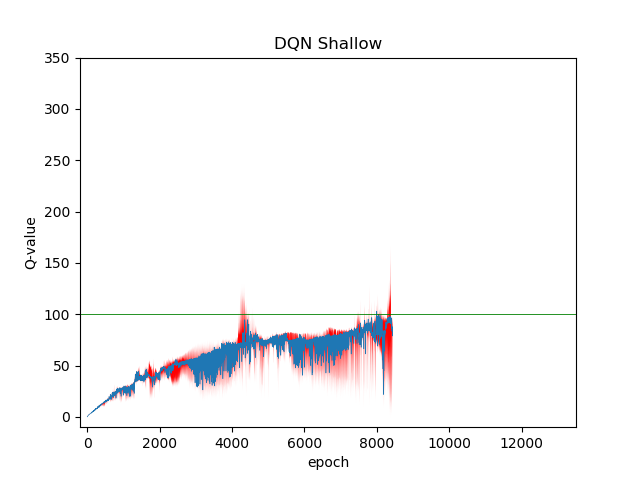
\includegraphics[width=.45\textwidth]{res/DQN_Shallow}} \quad
	\subfloat{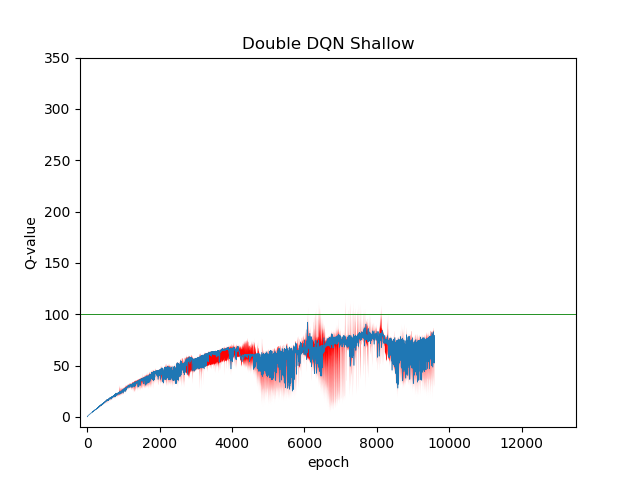
\includegraphics[width=.45\textwidth]{res/DoubleDQN_Shallow}} \\
	\subfloat{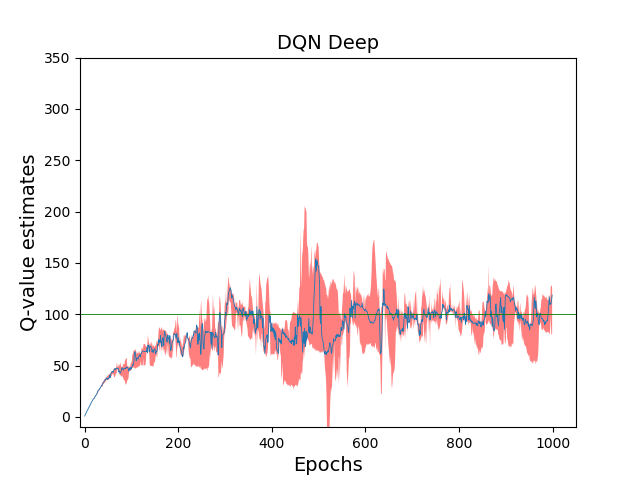
\includegraphics[width=.45\textwidth]{res/DQN_Deep}} \quad
	\subfloat{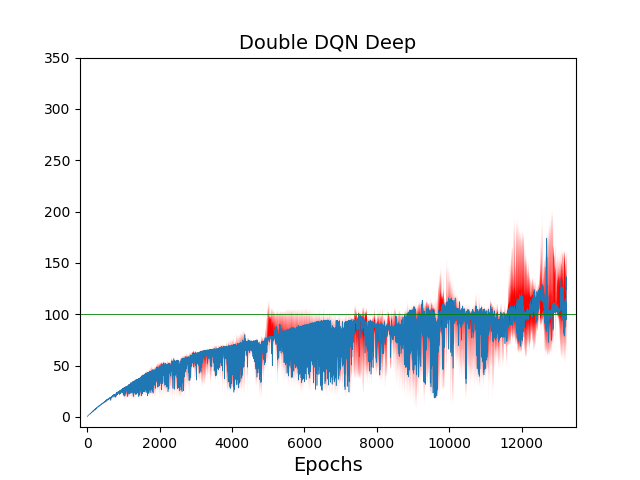
\includegraphics[width=.45\textwidth]{res/DoubleDQN_Deep}} \\
	
	%\subfloat[][\emph{Cascata}.]
	%{\includegraphics[width=.45\textwidth]{Cascata}} \quad
	%\subfloat[][\emph{Salita e discesa}.]
	%{\includegraphics[width=.45\textwidth]{SalitaDiscesa}}
	\caption{The blue lines in the figure represents the median of the q-value  per epoch (the average Q-value computed every 64 steps) from the executions of 3 seeds for each configuration. The red line shows the maximal and minimal oscillation of the results.}
	\label{fig:q-values}
\end{figure*}